%----------------------------------------------------------------------------------------
%	PACKAGES AND OTHER DOCUMENT CONFIGURATIONS
%----------------------------------------------------------------------------------------

\documentclass[11pt,spanish,a4paper]{article} % Default font size is 12pt, it can be changed here

\usepackage{geometry} % Required to change the page size to A4
\geometry{a4paper} % Set the page size to be A4 as opposed to the default US Letter

\usepackage{graphicx} % Required for including pictures
\usepackage{enumerate}
\usepackage{float} % Allows putting an [H] in \begin{figure} to specify the exact location of the figure
\usepackage{wrapfig} % Allows in-line images such as the example fish picture
\usepackage{setspace}
\usepackage{amsmath} % Matrix package
\setcounter{MaxMatrixCols}{25}
\usepackage{listings}
\usepackage{hyperref}

\usepackage{lipsum} % Used for inserting dummy 'Lorem ipsum' text into the template

\linespread{1.2} % Line spacing

%\setlength\parindent{0pt} % Uncomment to remove all indentation from paragraphs

\graphicspath{{./images/}} % Specifies the directory where pictures are stored

\usepackage[utf8]{inputenc}
\usepackage[spanish]{babel}

\begin{document}

%----------------------------------------------------------------------------------------
%	TITLE PAGE
%----------------------------------------------------------------------------------------

\begin{titlepage}

\newcommand{\HRule}{\rule{\linewidth}{0.5mm}} % Defines a new command for the horizontal lines, change thickness here

\center % Center everything on the page

\textsc{\LARGE Universitat Politècnica de València}\\[1.5cm] % Name of your university/college
\textsc{\Large Biometría}\\[2.5cm] % Major heading such as course name
\textsc{\large Máster en Inteligencia Artificial, Reconocimiento de Formas e Imagen Digital}\\[1.5cm] % Minor heading such as course title

\HRule \\[0.4cm]
{ \Huge \bfseries Viola and Jones para la\\\vspace{0.8em} detección de caras (C++)}\\[0.4cm] % Title of your document
\HRule \\[2.5cm]

\begin{minipage}{0.4\textwidth}
\begin{flushleft} \large
\emph{Autor:}\\
Alejandro \textsc{Pérez González de Martos}
\end{flushleft}
\end{minipage}
~
\begin{minipage}{0.4\textwidth}
\begin{flushright} \large
\emph{aperez@dsic.upv.es} \\
\end{flushright}
\end{minipage}\\[3cm]

{\large \today}\\[1cm] % Date, change the \today to a set date if you want to be precise

%\includegraphics{Logo}\\[1cm] % Include a department/university logo - this will require the graphicx package

\vfill % Fill the rest of the page with whitespace

\end{titlepage}

%----------------------------------------------------------------------------------------
%	TABLE OF CONTENTS
%----------------------------------------------------------------------------------------

\tableofcontents % Include a table of contents

\newpage % Begins the essay on a new page instead of on the same page as the table of contents 

%----------------------------------------------------------------------------------------
%	INTRODUCTION
%----------------------------------------------------------------------------------------

\section{Introducción} % Major section

En esta memoria se presentan los detalles sobre una implementación en C++ del \textit{framework} para la detección de objetos Viola and Jones. En concreto se ha empleado este framework para entrenar un detector de caras humanas. A continuación se presentan los detalles de la implementación, el funcionamiento del framework y el entrenamiento seguido para la construcción del detector de caras.

%------------------------------------------------

\section{Viola and Jones: implementación}

No es objeto de esta memoria presentar el framework Viola and Jones, sino ceñirse a los detalles de la implementación realizada. Por ello, en los siguientes apartados se asumirá que se conoce en buen grado el funcionamiento del mismo.

\subsection{Características Haar empleadas}

En la figura \ref{fig:features} se muestran las cuatro características tipo Haar empleadas en el framework. Se ha decidido prescindir de aquellas con más número de rectángulos debido a su dudosa utilidad para la detección de rostros humanos.

\begin{figure}[H]
\center{
\includegraphics[width=0.9\linewidth]{features}}
\caption{Características Haar empleadas}
\label{fig:features}
\end{figure}

Además se han impuesto una serie de restricciones en el tamaño de las características según su tipo con dos motivos fundamentales: evitar la sobreespecialización de las características sobre el conjunto de entrenamiento y reducir en gran medida el número de características global. Las restricciones son las siguientes:

\begin{itemize}
\item \textbf{A}: Tamaño mínimo 4x4 píxeles.
\item \textbf{B}: Tamaño mínimo 4x4 píxeles.
\item \textbf{C}: Tamaño mínimo 3x4 píxeles.
\item \textbf{D}: Tamaño mínimo 4x3 píxeles.
\end{itemize}

El número total de características a considerar en una ventana de 21x21 píxeles atendiendo a estas restricciones es 54720.

\subsection{Imagen Integral}

Las características Haar pueden ser calculadas rápidamente usando una representación intermedia de la imagen conocida como \textit{imagen integral}. La imagen integral en las coordenadas $x, y$ contiene el sumatorio de los píxeles que quedan encima y a la izquierda del actual (incluyendo $x, y$). Por ello, el framework carga en memoria únicamente la imagen integral de cada una de las muestras proporcionadas como conjunto de entrenamiento, pues la muestra original no es empleada con posterioridad.

\subsubsection{Sumar los valores de los píxeles en un rectángulo de la imagen usando la Imagen Integral}

\textbf{entrada:} La imagen integral $ii$ de una imagen $i$. Posición, altura $h$ y anchura $w$ de un rectángulo contenido en la imagen: $[x_0, x_{0}+w-1]$x$[y_0, y_{0}+h-1]$

\textbf{salida:} Sumatorio del valor de los píxeles contenidos en el rectángulo de tamaño $w$ x $h$ ($S$).

\begin{enumerate}\itemsep=-2mm
\item $S \leftarrow ii(x+w, y+h)$;
\item \textbf{if} $x_0 > 0$ \textbf{then} $S \leftarrow S-ii(x_0 - 1, y_0 + h - 1)$;
\item \textbf{if} $y_0 > 0$ \textbf{then} $S \leftarrow S-ii(x_0 + w - 1, y_0 - 1)$;
\item \textbf{if} $x_0 > 0$ \textbf{and} $y_0 > 0$ \textbf{then} $S \leftarrow S+ii(x_0 - 1, y_0 - 1)$;
\item \textbf{return} $S$;
\end{enumerate}

\subsection{Algoritmo AdaBoost}

El algoritmo AdaBoost implementado se encarga de seleccionar, en cada iteración, la característica Haar que proporciona el menor error \textit{ponderado} en clasificación sobre el conjunto de entrenamiento. El peso del error de cada muestra se actualiza en función de si la última característica obtenida ha sido capaz de clasificar correctamente dicha muestra o no, de forma que las siguientes características den más importancia a aquellas muestras que no han sido bien clasificadas por las anteriores.

En la implementación realizada, el algoritmo AdaBoost recibe, además de los conjuntos de muestras positivas, muestras negativas, muestras de validación y el conjunto total de características Haar, dos parámetros de entrada que determinan la condición de parada del entrenamiento del \textit{Strong Classifier} actual:

\begin{itemize}
\item \textbf{Mínimo FPR a alcanzar (minfpr):} mientras el FPR que proporciona el \textit{Strong Classifier} actual sobre las muestras negativas sea superior al \textit{minfpr}, se añadirá un nuevo \textit{Weak Classifier} (una nueva característica Haar y su \textit{threshold}) al mismo.
\item \textbf{Máximo FNR permitido (maxfnr):} el \textit{threshold} del \textit{Strong Classifier} se ajustará tras añadir un nuevo \textit{Weak Classifier} al mismo de forma que, como máximo, clasifique de forma errónea un $(maxfnr*100)\%$ del conjunto de muestras positivas.
\end{itemize}

A continuación se muestra en pseudocódigo el algoritmo AdaBoost implementado:

\begin{footnotesize}
\begin{itemize}
\item Dadas muestras de entrenamiento $(x_1,y_1), ..., (x_n, y_n)$ donde $y_i \in {0,1}$ para muestras negativas y positivas respectivamente, y los valores $minfpr, maxfnr$.
\item Inicializar los pesos de las muestras como $w_i = \frac{1}{2m}, \frac{1}{2l}$ para $y_i = 0, 1$ respectivamente, donde $m$ y $l$ son el número de muestras negativas y positivas respectivamente.
\item Inicializar un \textit{Strong Classifier} vacío (sin ningún \textit{Weak Classifier}).
\item Inicializar $FPR = 1.0$
\item Mientras $FPR > minfpr$:
  \begin{itemize}
  \item Normalizar los pesos, $w_i = \frac{w_i}{\sum_{\substack{j=1}}^{n}w_j}$.
  \item Para cada característica, $j$, entrenar un clasificador $h_j$ con la restricción de sólo poder usar la característica $j$. El error se evalúa respecto a $w$,\\$\epsilon_j = \sum_i w_i |h_j(x_i)-y_i|$.
  \item Seleccionar el clasificador $h_j$ que minimiza el error $\epsilon$.
  \item Actualizar los pesos de las muestras:\\\hspace*{3em}$w_i = w_i\beta^{1-e_i}$\\donde $e_i = 0$ si la muestra $x_i$ se clasifica correctamente y $e_i = 1$ si no, $\beta = \frac{\epsilon}{1-\epsilon}$ y $m$ es el número de muestras negativas.
  \item Añadir $h_j$ al \textit{Strong Classifier} con un peso $\alpha = log(\frac{1}{\beta})$.
  \item Ajustar el \textit{threshold} del \textit{Strong Classifier} tal que $FNR \leq maxfnr$, siendo\\\hspace*{3em}$FNR = \frac{\sum_i (1-e_i)}{l} \quad \forall i \rightarrow y_i = 1$.
  \item Calcular el FPR sobre el conjunto de validación \textit{(muestras negativas no pertenecientes al entrenamiento)}.
  \end{itemize}
\item El \textit{Strong Classifier} final es:\\\hspace*{3em}$h(x) = 1 \quad si \quad \sum_{\substack{t=1}}^T \alpha_t h_t(x) \geq threshold$\\\hspace*{3em}$h(x) = 0 \quad sino$.
\end{itemize}
\end{footnotesize}

\subsubsection{Algunos detalles de implementación}

\begin{itemize}
\item Ajuste del threshold del Weak Classifier para obtener el mínimo error de clasificación:

\vspace*{1em}El \textit{threshold} óptimo puede obtenerse en una sola pasada sobre una lista ordenada del valor que proporciona la característica Haar sobre cada muestra de entrenamiento. Para cada elemento de la lista se evalúan y almacenan cuatro sumatorios:

\begin{itemize}
\item $T^+$: el sumatorio de los pesos de todas las muestras positivas (fijo).
\item $T^-$: el sumatorio de los pesos de todas las muestras negativas (fijo).
\item $S^+$: el sumatorio de los pesos de todas las muestras positivas por debajo de la muestra actual.
\item $S^-$: el sumatorio de los pesos de todas las muestras negativas por debajo de la muestra actual.
\end{itemize}

El error para el threshold con valor igual al que proporcionó la característica Haar para la muestra actual es:

\[ \epsilon = min(S^{+} + (T^{-} - S^{-}), S^{-} + (T^{+} - S^{+})) \]

\item Ajuste del threshold del Strong Classifier en función del $FNR_{max}$ permitido por paso:

Se obtiene el valor proporcionado por el \textit{Strong Classifier} para todas las muestras positivas del conjunto de entrenamiento y se ordenan en función de este. Se selecciona como \textit{threshold} el valor de la muestra que ocupa la posición $FNR_{max} \cdot |P|$.

\end{itemize}

\subsection{Clasificador en cascada}

En esta sección se detalla el entrenamiento implementado del clasificador en cascada.

\begin{footnotesize}
\begin{itemize}
\item $P$, conjunto de muestras positivas.
\item $N$, conjunto de muestras negativas.
\item $V$, conjunto de muestras negativas para validación (opcional).
\item Parámetros (principales) seleccionados por el usuario:
  \begin{itemize}
  \item Ratio de falsos positivos objetivo $F_{target}$.
  \item Número de pasos del clasificador $S$.
  \item Máximo FNR por paso permitido $FNR_{max}$.
  \item Número máximo de muestras negativas por paso para el entrenamiento $n_{-}$.
  \end{itemize}
\item A partir de $S$ y $F_{target}$ se calcula el ratio de falsos positivos objetivo por paso $fpr_i$, de forma que:\[ \prod_{i=1}^{S} fpr_i = F_{target} \]
\item Generar un nuevo Cascade Classifier $CC$ que clasifique todas las muestras como positivas.
\item $N_i \leftarrow \emptyset$.
\item Para $i=1$ hasta $S$:
  \begin{itemize}
  \item Añadir muestras de $N$ a $N_i$ que $CC$ clasifique como positivas hasta que $|N_i| = n_{-}$.
  \item Entrenar un \textit{Strong Classifier} mediante AdaBoost $(P, N_i, V, fpr_i, FNR_{max})$ y añadirlo a $CC$.
  \item Eliminar de $P$ y $N_i$ las muestras clasificadas como negativas por $CC$.
  \end{itemize}
\end{itemize}
\end{footnotesize}

\subsection{Detección}

\subsubsection{Escalado}

En el modo de detección, el programa carga un clasificador en cascada previamente entrenado y almacenado para la detección de un tipo de objetos concreto. Puesto que estos objetos pueden variar en tamaño y posición dentro de la imagen fuente a escanear, es necesario correr ventanas de distintos tamaños alrededor de la imagen. Sin embargo, en principio nuestro clasificador en cascada está entrenado para detectar objetos de tamaño fijo usando unas características Haar muy concretas.

La ventaja que presentan este tipo de características es que son fácilmente escalables. Estas miden la diferencia de nivel de gris medio entre dos o más rectángulos de la imagen. Por tanto, para evaluar una región con, por ejemplo, el doble de píxeles que el tamaño original (en nuestro caso $42x42$ en lugar de $21x21$), lo único que tendremos que hacer es escalar las características acorde al nuevo tamaño de la ventana y modificar los \textit{threshold}s de los \textit{Weak Classifier}s:

\begin{itemize}
\item Factor de escalado $s$.
\begin{itemize}
\item $x = x \cdot s$
\item $y = y \cdot s$
\item $width = width \cdot s$
\item $height = height \cdot s$
\item $threshold = threshold \cdot s^2$
\end{itemize}
\end{itemize}

Dada una imagen para la detección, se prueban todos los posibles tamaños de ventana desde la resolución base de entrenamiento ($21x21$) hasta el tamaño total de la imagen, aumentando en un factor de escala por defecto de $1.25$ cada iteración.

\subsubsection{Post-normalización de valores en lugar de pre-normalización de ventanas}

Para detectar objetos sobre una imagen necesitamos correr ventanas de múltiples tamaños a lo largo de toda la imagen con el fin de abarcar todos los posibles tamaños y posiciones de los objetos a encontrar. Puesto que el sistema funciona sobre imagenes integrales de ventanas normalizadas a media $0$ y desviación típica $1$, sería necesario primero normalizar cada una de las ventanas y posteriormente calcular su imagen integral.

Sin embargo, es posible normalizar \textit{a posteriori} el valor que nos devuelve una característica Haar sobre una ventana sin normalizar en lugar de calcular el valor sobre la ventana normalizada. Para ello necesitaremos poder calcular, para una subventana dada, su media y su varianza. Estos dos valores son fácilmente calculables mediante dos imágenes integrales sobre la imagen completa. Recordemos que:

\[ \sigma^{2} = m^2 - \frac{1}{N} \sum x^2 \]

donde $\sigma$ es la desviación típica, $m$ es la media y $x$ es el valor del píxel de la ventana. La media de la ventana es fácilmente obtenible mediante la imagen integral normal, mientras que el sumatorio de los píxeles al cuadrado se obtiene haciendo uso de una imagen integral sobre los píxeles al cuadrado.

De este modo, la normalización se realiza sobre el valor obtenido por la característica Haar y no sobre cada ventana de la imagen, reduciendo de este modo el coste computacional de manera drástica. 

Este es sin duda el punto clave en el proceso de detección en Viola and Jones.

\section{Detección de caras}

\subsection{Conjunto de entrenamiento}

Disponemos de un conjunto de 6099 caras y otro de 10000 no-caras de tamaño 21x21 píxeles, ambos en escala de grises y normalizados a media 0 y desviación típica 1, disponibles en:

\vspace*{1em}
\url{http://users.dsic.upv.es/~rparedes/teaching/Biometria/index.html}
\vspace*{1em}

Para entrenar un clasificador en cascada adecuado para la detección de caras con un FPR en torno a $10^{-6}$, en [1] utilizan aproximadamente 350 millones de muestras negativas. Este número tan elevado se debe a que para entrenar la etapa $j$, las muestras de entrenamiento negativas empleadas deben ser \textit{incorrectamente} clasificadas como positivas por las $i=1$ hasta $j-1$ etapas anteriores ($N_i$ sólo contiene muestras \textit{potencialmente positivas}). Por tanto, si tenemos actualmente $S-1$ etapas entrenadas cuyo FPR global sobre el conjunto de validación es de $10^{-5}$, para entrenar la etapa $S$ harán falta aproximadamente $\frac{n_{-}}{10^{-5}}$ muestras negativas. Por ejemplo, para $n_{-} = 6000$ necesitaríamos $\frac{6000}{10^{-5}} = 6 \cdot 10^7$ muestras únicamente para entrenar la última etapa.

[1]: \textit{``With the cascaded detector, the final layers of the cascade may effectively look through hundreds of millions of negative examples in order to find a set of 10,000 negative examples that the earlier layers of the cascade fail on. So the negative training set is much larger and more focused on the hard examples for a cascaded detector''}.

Con el fin de generar un conjunto de muestras negativas suficientemente grande para el entrenamiento se ha implementado una utilidad que, dado un conjunto de imágenes (que no contengan caras) en formato \textit{png}, genera muestras negativas normalizadas de ventanas de tamaño especificable (en nuestro caso de 21x21) sobre la imagen.

Además, se ha implementado la rotación y el \textit{vertical mirroring} de imágenes con el fin de ampliar fácilmente el conjunto de entrenamiento:

\begin{itemize}
\item Se ha añadido el \textit{vertical mirror} de las caras al conjunto de muestras positivas, pues una cara vista en un espejo sigue siendo una cara (total $6099\cdot2 = 12198$).
\item Se ha añadido la rotación de 90, 180 y 270 grados de las muestras negativas al conjunto de muestras negativas.
\end{itemize}

\subsection{Parámetros empleados}

Los parámetros empleados para el entrenamiento del clasificador en cascada para la detección de caras han sido:

\begin{itemize}
\item Tamaño (máximo) del clasificador en cascada: 6
\item FPR global objetivo: $10^{-6}$
\item FPR objetivo por paso: 0.5 0.25 0.053183 0.053183 0.053183 0.053183
\item FNR máximo permitido por paso: 0.02
\item Número de muestras negativas para el entrenamiento por paso: 12198
\end{itemize}

El motivo de tener un clasificador de únicamente 6 etapas es que no se han recolectado suficientes muestras negativas para el entrenamiento de más etapas. Las aproximadamente dos millones de no-caras quedan rápidamente clasificadas correctamente en pocas etapas. Recordemos que en [1] emplean aproximadamente 350 millones.

\subsection{Resultados sobre los conjuntos de entrenamiento y validación}

\begin{itemize}
\item Conjunto de validación (10000 ventanas de no-caras + rotaciones):

\begin{verbatim}
Loading positive samples file (+ vertical mirror) ... OK (12198)
Loading negative samples file (+ 90, 180 and 270 deg.) ... OK (40000)

Cascade classifier total steps: 6

Cascade classifier best 3 features:
  #1 (Type Width Height X Y) = (2 12 4 5 3)
  #2 (Type Width Height X Y) = (1 4 4 15 5)
  #3 (Type Width Height X Y) = (0 4 4 7 1)

Cascade classifier performance:
  FN = 2211/12198, FP = 0/40000
\end{verbatim}

\item Conjunto de entrenamiento (2025727 ventanas de no-caras):

\begin{verbatim}
Loading positive samples file (+ vertical mirror) ... OK (12198)
Loading negative samples file ... OK (2025727)

Cascade classifier total steps: 6

Cascade classifier best 3 features:
  #1 (Type Width Height X Y) = (2 12 4 5 3)
  #2 (Type Width Height X Y) = (1 4 4 15 5)
  #3 (Type Width Height X Y) = (0 4 4 7 1)

Cascade classifier performance:
  FN = 2211/12198, FP = 0/2025727
\end{verbatim}

\end{itemize}

\subsection{Almacenamiento de los clasificadores en cascada}

Puesto que entrenar un clasificador en cascada es computacionalmente costoso es necesario almacenar los modelos una vez entrenados. Para ello se ha diseñado un formato simple capaz de almacenar todos los datos relativos a un clasificador en cascada, en concreto:

\begin{itemize}
\item Cascade Classifier:
  \begin{itemize}
  \item Resolución base de las muestras de entrenamiento.
  \item Número de \textit{Strong Classifier}s.
  \begin{itemize}
  \item De cada \textit{Strong Classifier}:
  \item Número de \textit{Weak Classifier}s.
  \item Threshold.
  \begin{itemize}
  \item De cada \textit{Weak Classifier}:
  \item Peso.
  \item Feature (tipo, ancho, alto, x, y).
  \item Threshold.
  \item Polaridad.
  \end{itemize}
  \end{itemize}
  \end{itemize}
\end{itemize}

\subsection{Resultados en un entorno real}

\begin{figure}[H]
\center{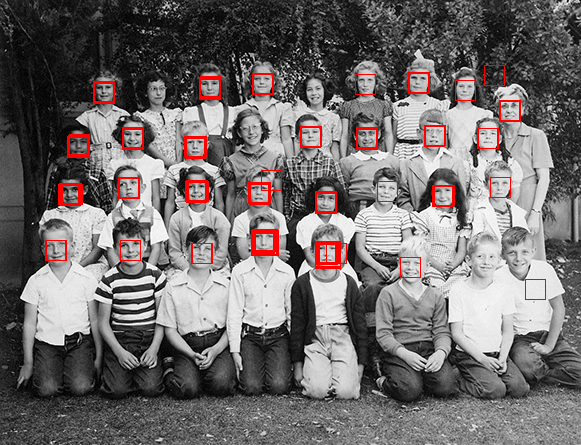
\includegraphics[width=0.9\linewidth]{class}}
\caption{Imagen 1}
\label{fig:det1}
\end{figure}

\begin{figure}[H]
\center{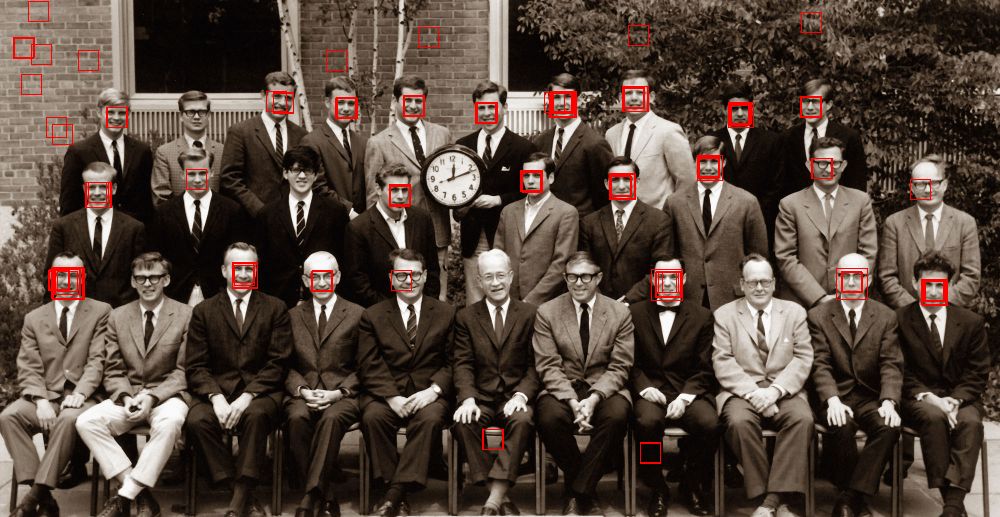
\includegraphics[width=0.9\linewidth]{edu}}
\caption{Imagen 2}
\label{fig:det2}
\end{figure}

\begin{figure}[H]
\center{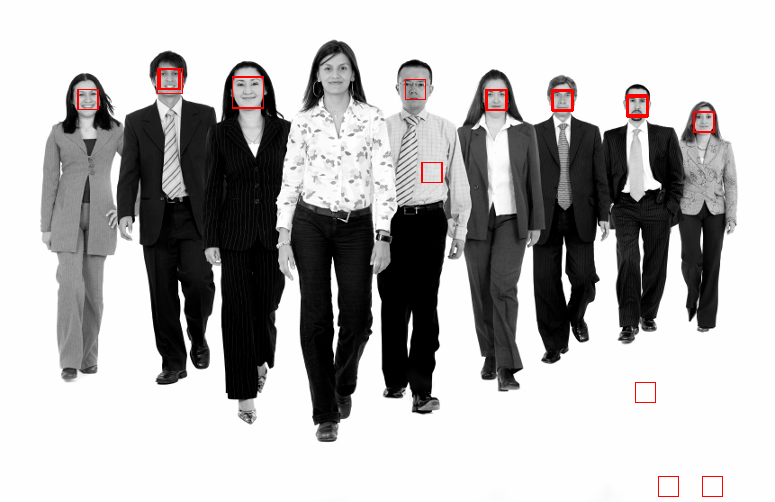
\includegraphics[width=0.9\linewidth]{people}}
\caption{Imagen 3}
\label{fig:det3}
\end{figure}

\section{Mejoras pendientes}

\begin{itemize}
\item Obtener más imágenes con muestras negativas para el entrenamiento.
\item Juntar detecciones solapadas.
\item \textit{Multithreading}.
\end{itemize}

\section{Uso del programa}

\begin{scriptsize}
\begin{lstlisting}
usage: ./lfobject

DETECTION
---------

  ./lfobject -m MODELFILE [--scale-step X --slide-step Y 
              --strictness S] IMAGE.PNG

    -m, --model MODEL.cc        cascade classifier trained model 
                                file for face detection
    --scale-step X	        sets scale factor step to X (default: 1.25)
    --slide-step Y              sets step between windows to Y*size(window) 
                                (default: 0.1)
    -s, --strictness S          reduces/increases strong classifiers threshold
                                on a factor S (default: 1.0)

TRAINING
--------

  ./lfobject -t --base-resolution B [--maxfnr-per-step M --cascade-steps S 
              --target-fpr T --negative-samples-per-step N --validation samples V
              --enable-rotation --disable-mirroring --verbose]
              --output OUTPUT.MODEL POS_SAMPLES_FILE NEG_SAMPLES_FILE 
              [VAL_NEG_SAMPLES_FILE]

    -t, --train		        generates a n-step cascade classifier using the 
                                modified AdaBoost algorithm.
    --base-resolution X		sets base resolution sub-window to 
                                X by X pixels (default: 21)
    -c, --cascade-steps S	sets cascade steps to S (default 8)
    --maxfnr-per-step M		sets maximum false negative ratio 
                                per step to M (default 0.01)
    --target-fpr T		sets target false positive ratio
                                to T (default 10^-6)
    --negative-samples-per-step sets maximum number of negative samples per
                                step (missclassified by previous stages)
    --validation-samples V      uses first V negative samples as validation set
    -o, --output OUTPUT.MODEL	URL of the output model file to be generated
    -v		                verbose

TEST
----

  ./lfobject --test -m MODELFILE [--strictness S --enable-rotation 
              --enable-mirroring] POS_SAMPLES_FILE NEG_SAMPLES_FILE
\end{lstlisting}
\end{scriptsize}

%----------------------------------------------------------------------------------------
%	BIBLIOGRAPHY
%----------------------------------------------------------------------------------------

\begin{thebibliography}{99} % Bibliography - this is intentionally simple in this template

\bibitem{BIB1}
Viola, P., \& Jones, M. J. (2004). 
\newblock Robust real-time face detection. 
\newblock International journal of computer vision, 57(2), 137-154.

\bibitem{BIB2}
Viola, P., \& Jones, M. (2001). 
\newblock Rapid object detection using a boosted cascade of simple features. 
\newblock In Computer Vision and Pattern Recognition, 2001. CVPR 2001. Proceedings of the 2001 IEEE Computer Society Conference on (Vol. 1, pp. I-511). IEEE.

\bibitem{BIB3}
OpenCV 2.4.7.0 Documentation
\newblock \url{http://docs.opencv.org/doc/user\_guide/ug\_traincascade.html}

\bibitem{BIB4}
Jensen, O. H. (2008). 
\newblock Implementing the Viola-Jones face detection algorithm.
\newblock (Doctoral dissertation, Technical University of Denmark, DTU, DK-2800 Kgs. Lyngby, Denmark).

\bibitem{BIB5}
Yi-Qing Wang (2013).
\newblock An Analysis of Viola-Jones Face Detection Algorithm.
\newblock IPOL Journal, Image Processing On Line.

\end{thebibliography}

%----------------------------------------------------------------------------------------

\end{document}
